\documentclass[conference]{IEEEtran}
\IEEEoverridecommandlockouts
\usepackage{cite}
\usepackage{amsmath,amssymb,amsfonts}
\usepackage{graphicx}
\usepackage{textcomp}
\usepackage{xcolor}
\usepackage{booktabs}
\usepackage{tabularx}
\usepackage{multirow}
\usepackage{array}
\usepackage{threeparttable}
\usepackage{stfloats}
\usepackage{url}
\usepackage{tikz}
\usetikzlibrary{positioning,arrows.meta,fit,shapes.geometric}

\graphicspath{{figures/}}
\renewcommand{\ttdefault}{cmtt}
\newcolumntype{Y}{>{\raggedright\arraybackslash}X}
\newcolumntype{P}[1]{>{\raggedright\arraybackslash}p{#1}}
\newcommand{\code}[1]{\texttt{\footnotesize #1}}
\makeatletter
\newcommand{\linebreakand}{\end{@IEEEauthorhalign}\hfill\mbox{}\par\mbox{}\hfill\begin{@IEEEauthorhalign}}
\makeatother

\begin{document}

\title{A Wearable-Driven Digital Twin for Monitoring Heart Failure Deterioration: Pulse-Based Physiological Simulation, Pre-Registered Scenario Testing and Real-Patient Replay}

\author{\IEEEauthorblockN{Kaveri Sharma}
\IEEEauthorblockA{\textit{Dept. of Computer Science Engg.}\\
\textit{PES University}\\
Bengaluru, India\\
kaveri05sharma@gmail.com}
\and
\IEEEauthorblockN{Mrunmayi Mohite}
\IEEEauthorblockA{\textit{Dept. of Computer Science Engg.}\\
\textit{PES University}\\
Bengaluru, India\\
mrunmayimohite9@gmail.com}
\and
\IEEEauthorblockN{Meghan Singhal}
\IEEEauthorblockA{\textit{Dept. of Computer Science Engg.}\\
\textit{PES University}\\
Bengaluru, India\\
meghansinghal@gmail.com}
\linebreakand
\IEEEauthorblockN{Adithya Balasubramanyam}
\IEEEauthorblockA{\textit{CAVE Labs, C-IoT, Dept. of CSE}\\
\textit{PES University}\\
Bengaluru, India\\
adithyakoundinya@gmail.com}
}

\maketitle

\begin{abstract}
Heart failure (HF) deteriorates gradually at home, yet monitoring remains episodic and consumer wearables report numbers without a model of what they mean physiologically. We present an end-to-end digital twin that couples home-measurable signals to a mechanistic physiology engine. A 21-day window of six wearable trends (resting heart rate, SpO$_2$, weight, steps, sleep, heart-rate variability) and routine clinical values (age, sex, BMI, ejection fraction, NT-proBNP) feed a Random Forest classifier and regressor that estimate one of five deterioration scenarios and its severity; these parameterize the Kitware Pulse engine through disease-specific cardiovascular modifiers; and a clinically anchored, interpretable risk score converts the simulated hemodynamic response into an alert, NYHA stage and 7/14/30-day projection, served through a FastAPI back end and React dashboard with day-to-day continuity of simulator state. On 300 held-out synthetic patients the classifier reached 90.7\% accuracy (macro-F1 0.91) and severity MAE 0.047; live re-validation through the deployed API gave severity MAE 0.026 (n=45). In a pre-registered test of ten scripted patient stories over 21 days and six seeds, the deployed alert detected three of five deteriorating patients and missed fluid overload and deconditioning, whose signatures do not reach the simulated hemodynamics; a component-guard rule reduced false alerts in stable patients by 61--68\% on development and held-out seeds without losing a detection. Replaying real home-monitoring data from 16 HF patients completed the full pipeline for 13. We document the engine instabilities, train/inference skews and integration faults encountered and how each was resolved, and we report real-outcome tests in which the twin's own scores were near chance, delimiting what the current design can and cannot claim.
\end{abstract}

\begin{IEEEkeywords}
Digital twin, heart failure, wearable sensors, physiology simulation, Pulse engine, random forest, remote patient monitoring, early warning, reproducibility.
\end{IEEEkeywords}

%=====================================================================
\section{Introduction}
%=====================================================================
Heart failure affects tens of millions of people worldwide \cite{james2018gbd,savarese2023burden} and is defined by progression: patients decline over days to weeks rather than instantaneously. Current guidelines emphasize early recognition of congestion and decompensation \cite{heidenreich2022}, yet three structural gaps remain in practice. First, monitoring is episodic: patients are typically seen every few weeks, and a patient can move from stable to crisis between visits. Second, consumer wearables report numbers, not physiology: a rising resting heart rate is measured, but whether it reflects benign variation or an early compensatory response to falling cardiac output is left to the patient. Third, threshold alarms (e.g., SpO$_2<92\%$) fire only after a value is already abnormal; they describe where a patient is, not where they are heading.

Remote monitoring has shown benefit when it captures physiology rather than symptoms alone, from structured telemonitoring \cite{inglis2008telemonitoring} to implanted pulmonary-artery pressure sensors \cite{abraham2011champion}, and multi-sensor wearables combined with machine learning have predicted HF hospitalization days in advance \cite{stehlik2020linkhf,gautam2022wearables}. These data-driven predictors, however, offer little mechanistic explanation of \emph{why} an alert fired. Cardiac digital twins promise exactly that mechanistic layer \cite{corral2020twin,coorey2022twin,niederer2021scaling}, but most are built from imaging or invasive measurements fitted to one patient at a time \cite{gu2025hftwin,geddes2025rhftwin}, and few are evaluated over weeks of everyday data.

This paper describes a digital twin that sits between these two traditions: it is driven by home-measurable wearable trends, interprets them through a mechanistic whole-body physiology engine (Kitware Pulse \cite{bray2019pulse}), and produces interpretable risk, staging and forward projections. Our contributions are:
\begin{enumerate}
\item A complete, open pipeline (wearable trends $\rightarrow$ ML scenario and severity estimation $\rightarrow$ Pulse simulation $\rightarrow$ interpretable risk scoring, NYHA staging and projection) deployed as a stateful web service with a clinician dashboard (Sections~\ref{sec:system}--\ref{sec:methods}).
\item Engine-level findings about using Pulse as a patient twin: how ejection fraction maps onto the engine, a root-caused instability boundary when disease modifiers and exertion are combined, and an exact state save/resume method that carries a patient's simulated physiology from day to day (Section~\ref{sec:engineering}).
\item A layered evaluation: offline and live model accuracy, a pre-registered 21-day scenario test with held-out seeds, replay of real home-monitoring data from HF patients, a two-patient ballistocardiography (BCG) check against measured hemodynamics, and real-outcome tests on two hospital cohorts (Section~\ref{sec:eval}).
\item A transparent account of the problems encountered and the solutions adopted, including negative results, so that the claims made are bounded by the evidence (Sections~\ref{sec:engineering}, \ref{sec:discussion}).
\end{enumerate}

%=====================================================================
\section{Related Work}\label{sec:related}
%=====================================================================
\textbf{Cardiac digital twins.} Corral-Acero \textit{et al.}\ \cite{corral2020twin} framed the digital twin as the route to precision cardiology, Coorey \textit{et al.}\ \cite{coorey2022twin} reviewed the emerging health-twin field for cardiovascular disease, and Niederer \textit{et al.}\ \cite{niederer2021scaling} argued that twins must move from artisanal, single-patient builds to scalable, industrial pipelines. Recent HF-specific twins fit mechanistic cardiovascular models to measured data: Gu \textit{et al.}\ \cite{gu2025hftwin} fitted twins to 343 HF patients and used the fitted parameters for interpretable phenotyping and prognosis, and Geddes \textit{et al.}\ \cite{geddes2025rhftwin} built CFD-based twins that non-invasively estimate markers of right HF. Balasubramanyam \textit{et al.}\ \cite{balasubramanyam2025twin} proposed a cardiovascular twin combining time-varying compliance, Fourier-based ECG reconstruction and 3D anatomical modeling.

\textbf{Wearable HF prediction.} The LINK-HF study \cite{stehlik2020linkhf} combined a wearable patch with machine learning to predict HF hospitalization with a median lead time of several days, and Gautam \textit{et al.}\ \cite{gautam2022wearables} surveyed AI, wearables and remote monitoring in HF. Invasive hemodynamic monitoring reduced HF hospitalization in the CHAMPION trial \cite{abraham2011champion}.

\textbf{Risk scores.} The MAGGIC score \cite{pocock2013maggic} is a widely used, externally validated HF survival score, and the LACE index \cite{vanwalraven2010lace} is a general readmission score; both serve as external benchmarks here.

\textbf{Positioning.} Table~\ref{tab:related} contrasts these approaches. Mechanistic twins personalize deeply but require hospital measurements; wearable predictors scale but are opaque. Our twin trades per-patient parameter fitting for deployability from home data, and adds a mechanistic layer that wearable-only predictors lack. We claim novelty for the integrated pipeline and its evaluation, not for any single component.

\begin{table*}[!t]
\centering
\caption{Positioning Against Related Work}
\label{tab:related}
\footnotesize
\begin{tabularx}{\textwidth}{@{}P{2.6cm}P{2.7cm}P{3.0cm}P{2.9cm}Y@{}}
\toprule
\textbf{Work} & \textbf{Input data} & \textbf{Model} & \textbf{Personalization} & \textbf{Gap addressed here} \\
\midrule
Corral-Acero 2020 \cite{corral2020twin}, Coorey 2022 \cite{coorey2022twin} & Multimodal (vision/review) & Mechanistic + statistical & Conceptual & No deployed system or longitudinal test \\
Gu 2025 \cite{gu2025hftwin} & Clinical, echo, invasive & Lumped cardiovascular model + unsupervised ML & Fitted per patient (343 HF) & Requires hospital measurements; no home monitoring \\
Geddes 2025 \cite{geddes2025rhftwin} & Imaging, invasive validation & 3D CFD & Fitted per patient & Right HF only; not wearable-driven \\
Balasubramanyam 2025 \cite{balasubramanyam2025twin} & ECG datasets, echo & Compliance model, Fourier ECG, 3D mesh & Signal-level & Visualization and ECG fidelity, not deterioration tracking \\
Stehlik 2020 (LINK-HF) \cite{stehlik2020linkhf} & Wearable patch & ML (similarity-based) & Patient baseline & No mechanistic explanation of alerts \\
\textbf{This work} & Wearable trends + routine clinical & RF + Pulse engine + interpretable score & Scenario/severity-driven, EF-scaled & Mechanistic, wearable-driven, evaluated over 21 days \\
\bottomrule
\end{tabularx}
\end{table*}

%=====================================================================
\section{System Overview}\label{sec:system}
%=====================================================================
Fig.~\ref{fig:arch} shows the pipeline. A patient record holds demographics and a clinical report (ejection fraction, NT-proBNP); daily wearable readings accumulate until a 21-day window is filled, which triggers one background assessment: (1) the scenario classifier and severity regressor (``Model~1''); (2) construction of a Pulse patient and scenario file; (3) simulation inside the Pulse container with crash and timeout detection; (4) hemodynamic feature extraction; (5) risk scoring, NYHA staging and trend-based deterioration rate; and (6) three further Pulse runs at projected severities for 7, 14 and 30 days. All results are persisted, so every read endpoint is a database read and never blocks on the engine. Table~\ref{tab:stack} lists the technology stack.

\begin{figure*}[!t]
\centering
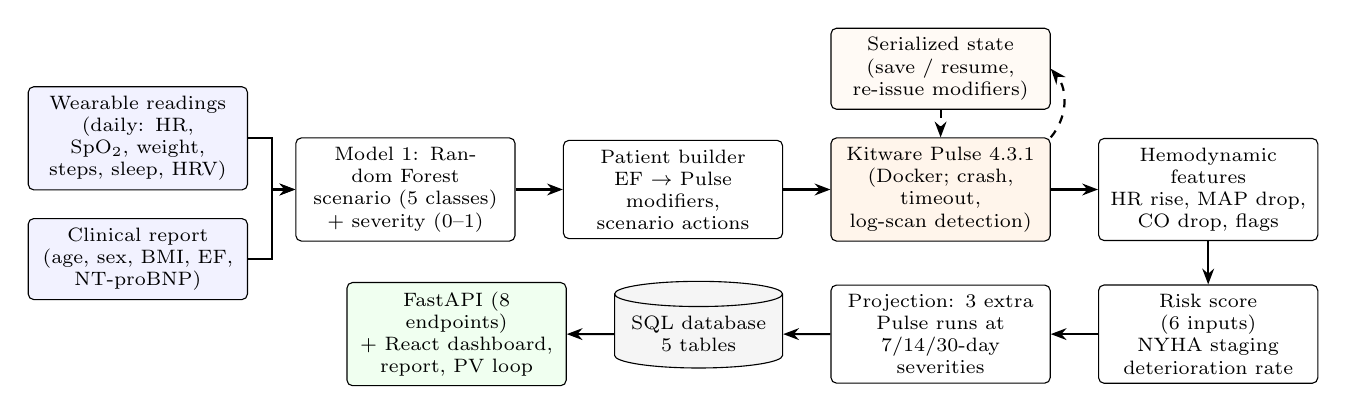
\begin{tikzpicture}[
  box/.style={draw, rounded corners=2pt, align=center, font=\scriptsize, minimum height=0.95cm, text width=2.55cm, fill=white},
  db/.style={draw, cylinder, shape border rotate=90, aspect=0.15, align=center, font=\scriptsize, minimum height=1.0cm, text width=1.9cm, fill=gray!8},
  arr/.style={-{Stealth[length=2mm]}, thick},
  lbl/.style={font=\scriptsize\bfseries, text=gray!60!black}]
\node[box, fill=blue!5] (w) {Wearable readings\\(daily: HR, SpO$_2$, weight,\\steps, sleep, HRV)};
\node[box, fill=blue!5, below=0.35cm of w] (c) {Clinical report\\(age, sex, BMI, EF,\\NT-proBNP)};
\node[box, right=0.6cm of w, yshift=-0.65cm] (m1) {Model 1: Random Forest\\scenario (5 classes)\\+ severity (0--1)};
\node[box, right=0.6cm of m1] (pb) {Patient builder\\EF $\rightarrow$ Pulse modifiers,\\scenario actions};
\node[box, right=0.6cm of pb, fill=orange!8] (pulse) {Kitware Pulse 4.3.1\\(Docker; crash, timeout,\\log-scan detection)};
\node[box, right=0.6cm of pulse] (feat) {Hemodynamic features\\HR rise, MAP drop,\\CO drop, flags};
\node[box, below=0.55cm of feat] (risk) {Risk score (6 inputs)\\NYHA staging\\deterioration rate};
\node[box, left=0.6cm of risk] (proj) {Projection: 3 extra\\Pulse runs at 7/14/30-day\\severities};
\node[db, left=0.6cm of proj] (dbn) {SQL database\\5 tables};
\node[box, left=0.6cm of dbn, fill=green!6] (ui) {FastAPI (8 endpoints)\\+ React dashboard,\\report, PV loop};
\node[box, above=0.35cm of pulse, fill=orange!4] (state) {Serialized state\\(save / resume,\\re-issue modifiers)};
\draw[arr] (w.east) -- ++(0.3,0) |- (m1.west);
\draw[arr] (c.east) -- ++(0.3,0) |- (m1.west);
\draw[arr] (m1) -- (pb); \draw[arr] (pb) -- (pulse); \draw[arr] (pulse) -- (feat);
\draw[arr] (feat) -- (risk); \draw[arr] (risk) -- (proj); \draw[arr] (proj) -- (dbn); \draw[arr] (dbn) -- (ui);
\draw[arr, dashed] (state) -- (pulse); \draw[arr, dashed] (pulse.north east) to[bend right=40] (state.east);
\end{tikzpicture}
\caption{System architecture. A filled 21-day wearable window triggers one background assessment; the dashed loop is the continuous-state mode, in which each day's simulation resumes from the previous day's serialized engine state (Section~\ref{sec:engineering}).}
\label{fig:arch}
\end{figure*}

\begin{table}[!t]
\centering
\caption{Technology Stack}
\label{tab:stack}
\footnotesize
\begin{tabularx}{\columnwidth}{@{}P{2.2cm}Y@{}}
\toprule
\textbf{Layer} & \textbf{Component} \\
\midrule
Physiology engine & Kitware Pulse 4.3.1 (\code{kitware/pulse:4.3.1} image, amd64) \cite{bray2019pulse} \\
Machine learning & scikit-learn 1.9.0 Random Forest \cite{breiman2001rf,pedregosa2011sklearn}; XGBoost 3.2.0 (secondary) \cite{chen2016xgboost} \\
Back end & Python 3.11, FastAPI, SQLAlchemy, Pydantic; SQLite (Postgres-portable) \\
Front end & React 19 + Vite; hand-built SVG charts \\
Deployment & Docker Compose (Postgres, back end, front end) \\
Testing & pytest (281 automated tests), Playwright browser checks, GitHub Actions CI \\
\bottomrule
\end{tabularx}
\end{table}

%=====================================================================
\section{Data}\label{sec:data}
%=====================================================================
\subsection{Reference data and synthetic training population}
No real patient data were used for training. Instead, every distribution parameter used by the synthetic generator is traced to an aggregate statistic from a real source (Table~\ref{tab:datasets}): MIMIC-IV HF admissions \cite{johnson2023mimiciv} for age, sex and laboratory values; the Chicco--Jurman HF clinical records \cite{chicco2020hf} as the only source with ejection fraction; and NHANES for height, weight and BMI by sex. A correlated generator produced $n=2{,}000$ synthetic patients across five scenarios, each with a 21-day wearable trajectory in one of three modes (stable, deteriorating, recovering). Only aggregate statistics from the real sources are stored in the repository; raw files remain outside version control.

Two candidate sources were rejected after inspection: a 5,000-row ``HF clinical records'' variant turned out to be a resampled copy of the same $\sim$300 patients (only 203 unique platelet values, 3,680 exact duplicate rows), and a public wearable dataset described as HF data contained general fitness data from 16 participants.

\begin{table}[!t]
\centering
\setlength{\tabcolsep}{3.5pt}\caption{Datasets and Their Roles}
\label{tab:datasets}
\footnotesize
\begin{tabularx}{\columnwidth}{@{}P{2.05cm}YP{1.95cm}@{}}
\toprule
\textbf{Source} & \textbf{Role} & \textbf{Access} \\
\midrule
MIMIC-IV \cite{johnson2023mimiciv} & Reference statistics; real-outcome test (17,129 HF ICU admissions) & PhysioNet credentialed \cite{goldberger2000physionet} \\
Chicco \& Jurman \cite{chicco2020hf} & EF, creatinine, sodium statistics & Public, CC BY 4.0 \\
NHANES & Height/weight/BMI by sex & Public survey \\
PerHeart \cite{kolakowski2026perheart} & Real home data, 27 HF patients aged 67--94; pipeline replay & Ethics-approved, Zenodo \\
Zigong HF cohort \cite{zhang2021zigong} & Real-outcome tests (2,001 admissions) & PhysioNet, DUA \\
Multi-pathology BCG \cite{zhan2025bcg} & Measured SV/CO for 2 patients & figshare \\
\bottomrule
\end{tabularx}
\end{table}

\subsection{Scenario taxonomy}
Five deterioration scenarios were fixed before modeling (Table~\ref{tab:scenarios}). Each maps to a specific set of Pulse actions, chosen so that the simulated physiology differs between scenarios rather than merely their labels.

\begin{table}[!t]
\centering
\setlength{\tabcolsep}{3.5pt}\caption{Scenario Taxonomy and Pulse Representation}
\label{tab:scenarios}
\footnotesize
\begin{tabularx}{\columnwidth}{@{}P{1.75cm}YP{2.55cm}@{}}
\toprule
\textbf{Scenario} & \textbf{Wearable signature} & \textbf{Pulse actions} \\
\midrule
stable & Flat trends & EF-derived modifiers only \\
fluid\_\allowbreak overload & Rising weight, rising HR & Venous compliance reduced with severity \\
cardiac\_stress & HR, HRV changes under exertion; preserved EF & Modifiers + \code{Exercise} \\
deconditioning & Falling steps, mild HR drift & Resistance/compliance modifiers; no exertion \\
acute\_\allowbreak deterioration & Rapid multi-signal decline; reduced EF & Modifiers + HR multiplier + \code{Exercise} \\
\bottomrule
\end{tabularx}
\end{table}

%=====================================================================
\section{Methods}\label{sec:methods}
%=====================================================================
\subsection{Model 1: scenario classifier and severity regressor}
Two Random Forests \cite{breiman2001rf} (300 trees, default depth) share one 29-column feature matrix: five clinical features (age, sex, BMI, EF, NT-proBNP) and, for each of six wearable signals, the first-7-day mean, last-7-day mean, their difference and the 21-day linear slope (24 features). The trend-mode column used during synthesis is dropped to prevent label leakage. Patients are split 70/15/15 (stratified by scenario) into training, validation and test sets.

\subsection{Personalizing Pulse}
Pulse does not accept ejection fraction as an input; EF is an output of its time-varying-elastance heart model. We therefore map EF and severity onto Pulse's \code{CardiovascularMechanicsModification} multipliers (stroke volume, systemic resistance and compliance, venous compliance, heart rate) and, for reduced EF, the binary \code{ChronicVentricularSystolicDysfunction} condition (a fixed elastance reduction). When the condition is applied, the continuous multiplier represents only the \emph{additional} acute severity, because stacking both produced cardiovascular collapse in validation. Pulse rejects patients outside age 18--65 and BMI 16--30; demographics are clamped only at the engine boundary, so the patient's true EF and severity still drive the simulation while the simulated body is a proxy.

\subsection{Hemodynamic features and risk score}
From each run we extract HR rise, MAP drop, cardiac-output (CO) drop, a compensation flag (stroke volume held $\geq95\%$) and an instability flag (MAP$_{\text{end}}<65$\,mmHg). The primary risk score (Table~\ref{tab:riskscore}) normalizes each to $[0,1]$ against a clinically anchored full scale and forms a weighted sum. During validation the score was structurally blind to fluid overload, whose danger appears as an already-congested baseline rather than an acute change, so a sixth input was added:
\begin{equation}
r=\max\big(\textstyle\sum_{i} w_i\, s_i,\; s_{\text{baseline}}(\text{MAP}_{\text{start}})\big),
\end{equation}
where $s_i$ are the five acute sub-scores and $s_{\text{baseline}}$ scores how far the simulated starting MAP lies below a healthy 92.5\,mmHg anchor. Buckets are LOW ($r<0.35$), MODERATE ($r<0.65$) and HIGH; these cut-points are an engineering choice, not a clinical citation. An XGBoost regressor \cite{chen2016xgboost} on the same features is kept as a secondary comparison only (5-fold CV MAE $0.089\pm0.020$, $R^2$ $0.828\pm0.091$; $n=117$ is too small to make it primary).

\begin{table}[!t]
\centering
\caption{Risk-Score Components and Clinical Anchors}
\label{tab:riskscore}
\footnotesize
\begin{tabularx}{\columnwidth}{@{}P{2.0cm}P{0.85cm}Y@{}}
\toprule
\textbf{Component} & \textbf{Weight} & \textbf{Anchor (citation)} \\
\midrule
HR rise & 0.15 & NEWS2 heart-rate bands \cite{rcp2017news2} \\
MAP drop & 0.20 & Healthy baseline to MAP 65\,mmHg \cite{vincent2013shock} \\
CO drop & 0.20 & 30\% decline = full scale \cite{nohria2002management,baran2019scai} \\
Compensation failure & 0.15 & Frank--Starling failure (binary) \\
Instability flag & 0.30 & MAP $<65$\,mmHg \cite{vincent2013shock} \\
Baseline deficit & max() & Starting MAP below 92.5\,mmHg anchor \\
\bottomrule
\end{tabularx}
\end{table}

\subsection{Staging, deterioration rate and projection}
NYHA staging is rule-based: AHA/ACC structural criteria (LVEF $\leq40\%$ or age-adjusted NT-proBNP above cut-off) \cite{heidenreich2022} gate whether symptoms have a structural basis, and the simulated exertion response places the patient in classes I--IV. A deterioration rate is computed from per-vital slopes normalized to population standard deviations per day; projection re-runs the full Pulse pipeline at linearly extrapolated severities for 7, 14 and 30 days.

\subsection{Service, alerts and continuous state}
The FastAPI service exposes eight endpoints over five tables (patients, clinical reports, wearable readings, simulation runs, risk assessments). Missing EF or NT-proBNP defaults to a documented healthy value (EF 62\%, NT-proBNP 100\,pg/mL), always flagged and never silently blended with measured values. A continuous-state mode serializes the Pulse engine state after each day and resumes from it the next day, instead of rebuilding the patient from scratch (Section~\ref{sec:engineering}).

%=====================================================================
\section{Engineering Challenges and Solutions}\label{sec:engineering}
%=====================================================================
Building the twin surfaced a series of problems that were not visible from documentation or offline evaluation. Table~\ref{tab:problems} summarizes them; the most consequential are detailed below.

\begin{table*}[!t]
\centering
\caption{Problems Encountered, Root Causes and Solutions}
\label{tab:problems}
\footnotesize\sloppy
\begin{tabularx}{\textwidth}{@{}P{3.1cm}YYP{2.6cm}@{}}
\toprule
\textbf{Problem} & \textbf{Root cause (how found)} & \textbf{Solution} & \textbf{Evidence} \\
\midrule
Pulse rejected scenario files & Actions/conditions need \code{PatientAction}/\code{AnyCondition} wrappers; found from protobuf parse errors & Builders emit the wrapped schema & All 5 scenarios run \\
Runs exited 1 with time mismatch & \code{CardiovascularMechanicsModification} without \code{Incremental:true} silently re-stabilizes, consuming extra time & Set \code{Incremental:true} & Clean exit, exact end time \\
Collapse at low EF (negative chamber volume) & Binary EF condition stacked with a second EF-derived cut & Continuous multiplier carries only the additional acute severity & Collapse no longer occurs \\
Real patients outside Pulse range & Engine hard-rejects age $>65$, BMI $>30$; real HF cohorts are older & Clamp demographics only at the engine boundary; flag per patient & 16/16 PerHeart patients flagged \\
Deconditioning looked like cardiac stress & Both used \code{Exercise}; HR 150--164 in both & Removed exertion from deconditioning & Distinct HR/MAP profiles (Table~\ref{tab:phase2}) \\
Fluid overload always scored LOW & Risk only measured change within a run; fluid overload is a shifted baseline & Added baseline-deficit term with \code{max()} & 30/30 LOW $\rightarrow$ 29/30 MODERATE \\
Live severity error 0.271 vs.\ 0.048 offline & NYHA ordinal used in training but unknown at inference, defaulted to class I & Removed NYHA from features; retrained & Live MAE 0.271 $\rightarrow$ 0.026 \\
Engine crashes at high severity & Disease modifiers + sustained exertion exceed engine's sustainable load (Table~\ref{tab:crashinv}) & Characterized; failures recorded, never dropped & Deterministic at 154.1--154.3\,s \\
Timeouts at 180\,s & Some runs need $\approx$180\,s under arm64 emulation & Documented margin; 2-worker cap & Re-attempts at 180.3--180.4\,s \\
Failures under concurrency & SQLAlchemy pool (5+10) exhausted; CPU contention & Concurrency 9 $\rightarrow$ 4 $\rightarrow$ 2 & 0 failures at 2 workers \\
Resumed state drifted & Disease modifiers are not carried by serialized state & Re-issue modifiers on every resume & Drift 6.5\% $\rightarrow$ 0.000\% \\
Engine segfault in continuous mode & Pulse Python SDK \code{initialize\_engine()} crash (gdb trace); earlier ``thread conflict'' diagnosis disproved & Switched to the CLI scenario driver & Day 1$\rightarrow$3 runs clean \\
Resumed runs flagged as crashes & Driver's end-time check ignores elapsed state time; schema field renamed (\code{Mode}, not \code{Type}) & Resume-aware crash filter; corrected schema & Exact match vs.\ continuous \\
Corrupted Pulse image & Local containerd-snapshotter extraction bug & Disabled snapshotter, re-pulled & Engine verified \\
Python 3.9 container errors & PEP 604 unions evaluated at class definition by SQLAlchemy/Pydantic & \code{Optional[...]} in model/schema files & Imports succeed \\
Dashboard could not call API & Browser enforces CORS (invisible to curl/TestClient) & CORS middleware (local only) & Found in browser test \\
Model drift across machines & Unpinned scikit-learn/numpy versions & Exact dependency pins; model SHA-256 checked before each run & Zero version warnings \\
SpO$_2$ output always 0.0 & Unresolved; likely emulation artifact & Never used as a feature & Excluded \\
ECG looked computed & Pulse ECG is a stored template scaled by HR & Labeled display-only in UI/API & Caveat in every response \\
\bottomrule
\end{tabularx}
\end{table*}

\subsection{Pulse instability at high severity}
In a 150-patient batch (30 per scenario), 117 runs completed (Fig.~\ref{fig:batch}). All 33 failures occurred in the two scenarios that add an \code{Exercise} action; 30 were engine crashes and 3 were timeouts, and failed patients had high severity (mean 0.75 and 0.72), so missingness is \emph{not at random} with respect to severity. Engine logs for three independent crashes showed an identical chain: fatigue, hypoxia and tachycardia, then renal hypoperfusion and cardiovascular collapse, ending in a fatal negative heart-chamber volume and an irreversible-state event at 154.1--154.3\,s. Table~\ref{tab:crashinv} lists single-variable interventions on a reproducible case. Gaps and ramps only delayed the crash; either stressor alone completed. The failure is therefore a sustained combined-load boundary whose safe exercise intensity varies by patient (about 0.22 for one patient and between 0.125 and 0.25 for another), so no single safe constant exists.

\begin{figure}[!t]
\centering
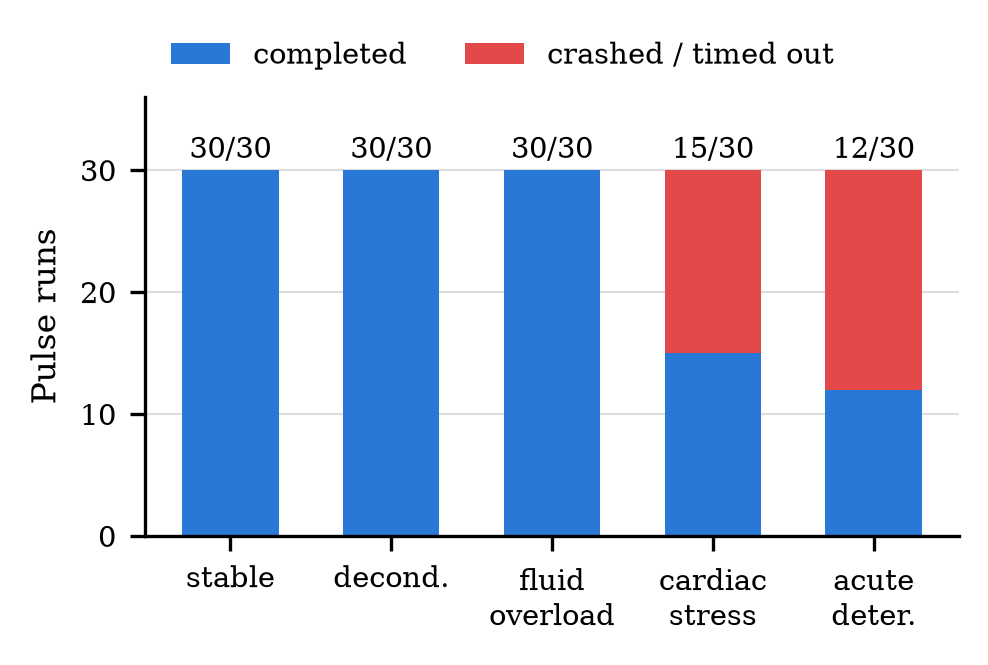
\includegraphics[width=\columnwidth]{fig_batch_success.png}
\caption{Pulse batch completion by scenario (150 runs). All failures occur in the two scenarios that combine disease modifiers with an \code{Exercise} action.}
\label{fig:batch}
\end{figure}

\begin{table}[!t]
\centering
\caption{Isolation Experiments on a Reproducible Crash (Severity 0.731)}
\label{tab:crashinv}
\footnotesize
\begin{tabularx}{\columnwidth}{@{}YP{2.3cm}@{}}
\toprule
\textbf{Intervention} & \textbf{Outcome} \\
\midrule
Control (exact reproduction) & Crash at 154.32\,s \\
60\,s gap before exertion & Crash at 212.02\,s \\
120\,s gap before exertion & Crash at 272.92\,s \\
Exertion ramped in 4 steps & Crash at 301.14\,s \\
Exertion alone, no disease modifiers & Completes (660\,s) \\
Disease modifiers alone, no exertion & Completes (660\,s) \\
Exertion intensity halved & Completes (660\,s) \\
\bottomrule
\end{tabularx}
\end{table}

\subsection{Two failure mechanisms with opposite character}
Failures were not a single phenomenon. Mechanism 1 (engine crash) depends on the patient's own severity and is deterministic, so retrying an identical scenario does not help. Mechanism 2 (timeouts and connection-pool exhaustion) depended on how many other patients were running: at 9 workers, 5/11 patients hit connection timeouts and 6/11 hit the 180\,s engine timeout; at 4 workers 8/11 still timed out; at 2 workers there were no failures. A bare completion rate conflates the two; we report the mechanism with each rate.

\subsection{Continuous state: carrying a patient forward}
Rebuilding a patient every day discards the physiological state the twin is meant to track. Pulse can serialize its full state (about 2.33\,MB, saved in 0.31--0.44\,s and loaded in 0.43\,s) and resume it, and with an \code{Exercise} action resumption was bit-for-bit identical to an uninterrupted run. With the disease modifier used by our pipeline it was not (Table~\ref{tab:resume}): the modifier is not carried by the serialized state. Re-issuing it on every resume restored an exact match, which also requires storing the last-used EF and severity alongside the state. A later end-to-end test crashed inside the Pulse Python SDK; isolating it showed a native crash in the SDK's engine initialization even with no machine-learning code loaded, disproving an earlier thread-conflict diagnosis, so the feature was rebuilt on the command-line driver.

\begin{table}[!t]
\centering
\setlength{\tabcolsep}{4pt}\caption{State Resume Fidelity (Patient EF 56.4, Severity 0.46; Final Values at 240\,s)}
\label{tab:resume}
\footnotesize
\begin{tabular}{@{}lrrrr@{}}
\toprule
\textbf{Run} & \textbf{HR} & \textbf{MAP} & \textbf{CO} & \textbf{SV} \\
\midrule
Continuous (reference) & 74.13 & 95.22 & 6.145 & 82.89 \\
Resumed, modifier not re-issued & 71.51 & 95.34 & 5.743 & 80.32 \\
\quad difference & $-3.5\%$ & $+0.1\%$ & $-6.5\%$ & $-3.1\%$ \\
Resumed, modifier re-issued & 74.13 & 95.22 & 6.145 & 82.89 \\
\quad difference & 0.000\% & 0.000\% & 0.000\% & 0.000\% \\
Two continuous runs (control) & \multicolumn{4}{c}{identical} \\
\bottomrule
\end{tabular}
\end{table}

\subsection{Other modeling corrections}
Three further corrections followed from running the real system rather than offline checks. (i) Severity (classifier output) and risk score (simulation-derived) share a $[0,1]$ range but not a scale: for acute deterioration the risk score's minimum (0.491) exceeded the severity mean (0.385). The projection module had applied a risk-score calibration to severity; the two calibrations were separated and the two quantities are now reported side by side, never fused. (ii) The classifier's label occasionally flipped between days for genuinely ambiguous trajectories; a categorical persistence rule (window chosen by sweep) now stabilizes the reported scenario. (iii) An attempt to add rolling-window curvature features (``Option A'') kept accuracy flat (90.7\%) but worsened severity MAE from 0.0473 to 0.0506 on held-out data, so it was reverted.

%=====================================================================
\section{Evaluation}\label{sec:eval}
%=====================================================================
We evaluate in layers of increasing realism. Table~\ref{tab:evalsummary} summarizes what each layer tests and what it does not.

\begin{table*}[!t]
\centering
\caption{Evaluation Layers and Their Scope}
\label{tab:evalsummary}
\footnotesize
\begin{tabularx}{\textwidth}{@{}P{3.2cm}P{3.6cm}YP{3.4cm}@{}}
\toprule
\textbf{Layer} & \textbf{Data} & \textbf{Main result} & \textbf{Does not test} \\
\midrule
Offline model test & 300 held-out synthetic patients & 90.7\% accuracy, severity MAE 0.047 & Real patients \\
Engine scenario check & 5 synthetic patients in Pulse & Physiologically distinct scenario responses & Clinical accuracy \\
Live API validation & 25 then 45 synthetic patients via live API & 25/25 completed; live MAE 0.026 after fix & Real patients \\
Pre-registered scenario test & 10 scripted stories $\times$ 6 seeds $\times$ 21 days & 3/5 deteriorations detected; false alerts cut 61--68\% & Real deterioration events \\
Real-patient replay & PerHeart, 16 HF patients & 13/16 completed end to end & Outcomes; patients' own physiology (age proxy) \\
BCG hemodynamics & 2 patients, measured SV/CO & Simulated CO 45--46\% below measured & Cohort-level accuracy; trends \\
Real-outcome tests & MIMIC-IV, Zigong & Twin's own scores near chance & Day-by-day early warning \\
\bottomrule
\end{tabularx}
\end{table*}

\subsection{Offline model accuracy}
On the 300-patient held-out test set, the classifier reached 90.7\% accuracy (macro-F1 0.91) and the regressor severity MAE 0.047 (RMSE 0.061). Cardiac stress (preserved EF) and acute deterioration (reduced EF), the pair hardest to separate from simulated HR/MAP alone, were cleanly separated because EF is an input. Removing all 24 wearable features cost 40 points of accuracy (Table~\ref{tab:ablation}), confirming that the wearable trend, not the clinical snapshot, carries most of the signal. The earlier 92.3\% figure belonged to a version that included NYHA class, removed for the reason in Table~\ref{tab:problems}.

\begin{table}[!t]
\centering
\setlength{\tabcolsep}{4pt}\caption{Model 1 on 300 Held-Out Synthetic Patients}
\label{tab:ablation}
\footnotesize
\begin{tabular}{@{}lccc@{}}
\toprule
\textbf{Variant} & \textbf{Accuracy} & \textbf{Severity MAE} & \textbf{RMSE} \\
\midrule
With NYHA feature (superseded) & 92.3\% & 0.048 & 0.063 \\
\textbf{Production (clinical + wearable)} & \textbf{90.7\%} & \textbf{0.047} & \textbf{0.061} \\
+ curvature features (reverted) & 90.7\% & 0.051 & 0.065 \\
Clinical features only & 50.3\% & 0.171 & 0.219 \\
\bottomrule
\end{tabular}
\end{table}

\subsection{Engine-level scenario validation}
Each scenario was simulated for one patient at severity $\approx$0.5 (Table~\ref{tab:phase2}). Responses were physiologically distinct. The clearest contrast is between cardiac stress and acute deterioration: both raised heart rate, but the healthy heart (EF 67\%) raised cardiac output from 5,910 to 9,948\,mL/min with stroke volume maintained, while the failing heart (EF 26.6\%) could not increase stroke volume (63$\rightarrow$67\,mL) and MAP fell to 52\,mmHg. This contrast was not tuned; it emerged from the EF-driven modifiers. The engine's left-heart pressure--volume signal was also physiologically plausible (volume 62.2--143.0\,mL, pressure 5.8--136.8\,mmHg at EF 45\%) and is shown on the dashboard as a PV loop.

\begin{table}[!t]
\centering
\caption{Simulated Response by Scenario (Severity $\approx$0.5)}
\label{tab:phase2}
\footnotesize
\begin{tabularx}{\columnwidth}{@{}P{1.7cm}ccY@{}}
\toprule
\textbf{Scenario} & \textbf{HR (bpm)} & \textbf{MAP (mmHg)} & \textbf{Note} \\
\midrule
stable & 71$\rightarrow$70 & 95$\rightarrow$95 & Flat \\
deconditioning & 71$\rightarrow$74 & 95$\rightarrow$95 & Mild drift \\
fluid\_overload & 72$\rightarrow$72 & 77$\rightarrow$77 & Congested baseline; CO +13\% \\
cardiac\_stress & 71$\rightarrow$164 & 95$\rightarrow$67 & Healthy compensation (EF 67\%) \\
acute\_deter. & 72$\rightarrow$132 & 78$\rightarrow$52 & SV cannot rise (EF 26.6\%) \\
\bottomrule
\end{tabularx}
\end{table}

\subsection{Live API validation}
Twenty-five synthetic patients (five per scenario) were replayed day by day through the live API with no mocking: 25/25 completed and all 25 were classified correctly, but severity MAE was 0.271, far from the offline 0.048. Per-patient inspection showed predictions compressed into a narrow 0.02--0.19 band, traced to the NYHA train/inference skew. After removing the feature and retraining, live re-validation reached severity MAE 0.008 on five patients and, expanded to 50 attempted (45 completed), MAE 0.0264 (95\% bootstrap CI 0.0194--0.0352) with 100\% scenario accuracy. The five failures were all high-severity exertion scenarios, matching Mechanism~1.

\subsection{Pre-registered 21-day scenario test}
Ten patient stories were written and their expected outcomes committed before any simulation (Table~\ref{tab:cohort}): five should be caught, three should stay quiet and two are edge cases. Each story was run for 21 days in continuous-state mode on development seeds 42--44 and, after a rule was selected, on held-out seeds 45--47. A pilot run exposed a design confound (EF matched to story severity) and two harness bugs (day-to-day noise scaled to the current value instead of the population SD, and per-process salting of Python's \code{hash()} making seeds non-reproducible); all were fixed and the harness was frozen before the main runs, with every amendment recorded.

\begin{table}[!t]
\centering
\caption{Pre-Registered Scenario Cohort}
\label{tab:cohort}
\footnotesize
\begin{tabularx}{\columnwidth}{@{}P{0.55cm}YP{1.9cm}@{}}
\toprule
\textbf{ID} & \textbf{Story} & \textbf{Group} \\
\midrule
P01 & Stable patient, ordinary life & stay quiet \\
P02 & Salty weekend (weight bump, recovers) & edge case \\
P03 & Slow, quiet weight gain & edge case \\
P04 & Fluid overload building (sev.\ 0.20$\rightarrow$0.50) & catch \\
P05 & Gradual deconditioning (sev.\ 0.20$\rightarrow$0.35) & catch \\
P06 & Cardiac stress, exertion episodes & catch \\
P07 & Sudden deterioration, days 10--13 & catch \\
P08 & Stressful fortnight, healthy heart & stay quiet \\
P09 & Active, stable patient & stay quiet \\
P10 & Everything goes wrong (sev.\ 0.20$\rightarrow$0.45) & catch \\
\bottomrule
\end{tabularx}
\end{table}

\textbf{Two alert definitions.} The first analysis alerted on the classifier's severity ($>0.15$) and caught all five deteriorating patients, but also alerted on all three stable ones (58.7 false alerts per 100 patient-days). A code audit then showed that the dashboard did not use this signal at all: it displayed the risk-score bucket (HIGH). Re-analysed under the dashboard's definition, the system detected three of five deteriorating patients (P06, P07, P10) with 18.0 false alerts per 100 patient-days. P05 (deconditioning) produced near-zero values on every risk component on all 63 patient-days, and P04 (fluid overload) did not congest in some seeds, so neither had any signal for an alert rule to act on.

\textbf{Alert rule selection.} Three candidate rules were specified before computing any of them (Fig.~\ref{fig:alerts}, Table~\ref{tab:alerts}). C3 downgrades a sustained HIGH that is driven only by the baseline-deficit term with no corroborating instability, the diagnosed cause of P08's persistent false alarm. It kept all three detections and cut false alerts by 67.6\% on development seeds and 61.4\% on held-out seeds, where it was never tuned.

\textbf{Unified alert decision.} The two alert signals were then merged into a single \code{decide\_alert()} function, which is now the only source of alert state in the API and dashboard. It has three levels: ALERT (risk bucket HIGH and not downgraded by C3, or a crashed/failed engine run via the classifier-severity fallback); WATCH (risk bucket MODERATE, or a HIGH streak that C3 downgrades); and NONE. C3 therefore downgrades but never silences: a HIGH risk bucket can never map to NONE. Replaying the saved scenario-test runs through the deployed functions reproduced the detection pattern on both seed sets (P06, P07 and P10 at ALERT in every seed; P01 and P09 quiet in every seed). P08's false alarm, previously ALERT for 8--14 consecutive days, was reduced to about 3 ALERT days per seed, with the remaining elevated days shown as WATCH. For P04 held-out seed 47, which never reached HIGH, 20 of 21 days now read WATCH, making a previously invisible fluid-overload trajectory visible for the first time.

\begin{figure}[!t]
\centering
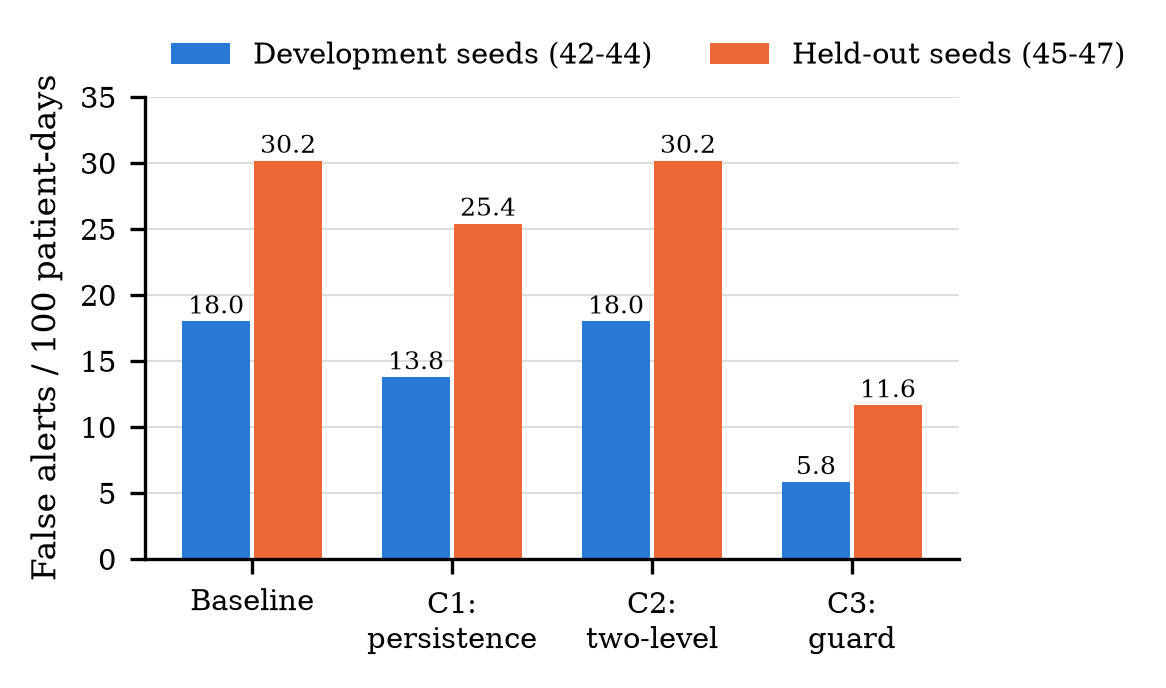
\includegraphics[width=\columnwidth]{fig_alert_candidates.png}
\caption{False alerts in the stay-quiet group per alert rule. C3 was selected on development seeds and confirmed on held-out seeds.}
\label{fig:alerts}
\end{figure}

\begin{table}[!t]
\centering
\caption{Alert Rules: Detections and False Alerts}
\label{tab:alerts}
\footnotesize
\begin{tabularx}{\columnwidth}{@{}Ycccc@{}}
\toprule
& \multicolumn{2}{c}{\textbf{Dev.\ (42--44)}} & \multicolumn{2}{c}{\textbf{Held-out (45--47)}} \\
\cmidrule(lr){2-3}\cmidrule(l){4-5}
\textbf{Rule} & \textbf{Caught} & \textbf{FA/100} & \textbf{Caught} & \textbf{FA/100} \\
\midrule
Baseline (risk bucket HIGH) & 3/5 & 17.99 & 3/5 & 30.16 \\
C1: HIGH for 3 consecutive days & 3/5 & 13.76 & 3/5 & 25.40 \\
C2: add sustained-MODERATE watch & 3/5 & 17.99 & 3/5 & 30.16 \\
\textbf{C3: component guard} & \textbf{3/5} & \textbf{5.82} & \textbf{3/5} & \textbf{11.64} \\
\bottomrule
\end{tabularx}
\end{table}

\textbf{Why false alerts occur.} Feature importances show the severity regressor relies on resting-HR delta and slope (63.2\% combined) and step-count trends (27.2\%), the signals that ordinary day-to-day variation moves most, while EF ranks tenth (0.6\%). Adding Gaussian noise at one population SD to a stable patient's window moved predicted severity from 0.11 to 0.43, crossing the stable-range threshold (Table~\ref{tab:noise}). A follow-up analysis also found that the cohort's neutral EF band (48--57\%) sits below the training ``stable'' class's EF range (51.3--70.7\%) and near the deconditioning mean, so day-by-day scenario-label accuracy on this cohort was only 17.6\% (222/1,260 patient-days), against 90.7\% on the in-distribution test set.

\begin{table}[!t]
\centering
\caption{Sensitivity of Predicted Severity to Added Wearable Noise}
\label{tab:noise}
\footnotesize
\begin{tabular}{@{}lcccc@{}}
\toprule
\textbf{Patient} & \textbf{0$\times$SD} & \textbf{1$\times$SD} & \textbf{1.5$\times$SD} & \textbf{2$\times$SD} \\
\midrule
P01 (stable) & 0.115 & 0.428 & 0.544 & 0.560 \\
P10 (deteriorating) & 0.777 & 0.570 & 0.622 & 0.850 \\
\bottomrule
\end{tabular}
\end{table}

\subsection{Real-patient replay (PerHeart)}
The PerHeart pilot dataset \cite{kolakowski2026perheart} contains one month of real home measurements (pulse oximeter, scale, blood-pressure cuff) from 27 HF patients aged 67--94. Sixteen had at least 21 real overlapping days of heart rate, SpO$_2$ and weight; no day was fabricated, and unmeasured fields (sleep, HRV, steps, EF, NT-proBNP) took documented defaults with explicit flags. Every patient required the engine's age proxy. Before the severity fix, all 16 completed but severities were compressed (0.078--0.148) and no patient reached HIGH, independently reproducing the NYHA skew on real data. After the fix (Fig.~\ref{fig:perheart}), severities spread (0.093--0.516) and five patients reached HIGH, while three patients now crashed with the deterministic engine signature. All 16 were staged NYHA~I, an artifact of the identical healthy EF/BNP defaults rather than a clinical finding. The one fluid-overload patient scored LOW because the EF default makes Pulse simulate a structurally normal heart, so the baseline-deficit term cannot fire; the API now names this mechanism in its caveat. We searched the literature for a BNP-to-EF proxy and found none: the clinical relationship runs from EF to BNP, not the reverse.

\begin{figure}[!t]
\centering
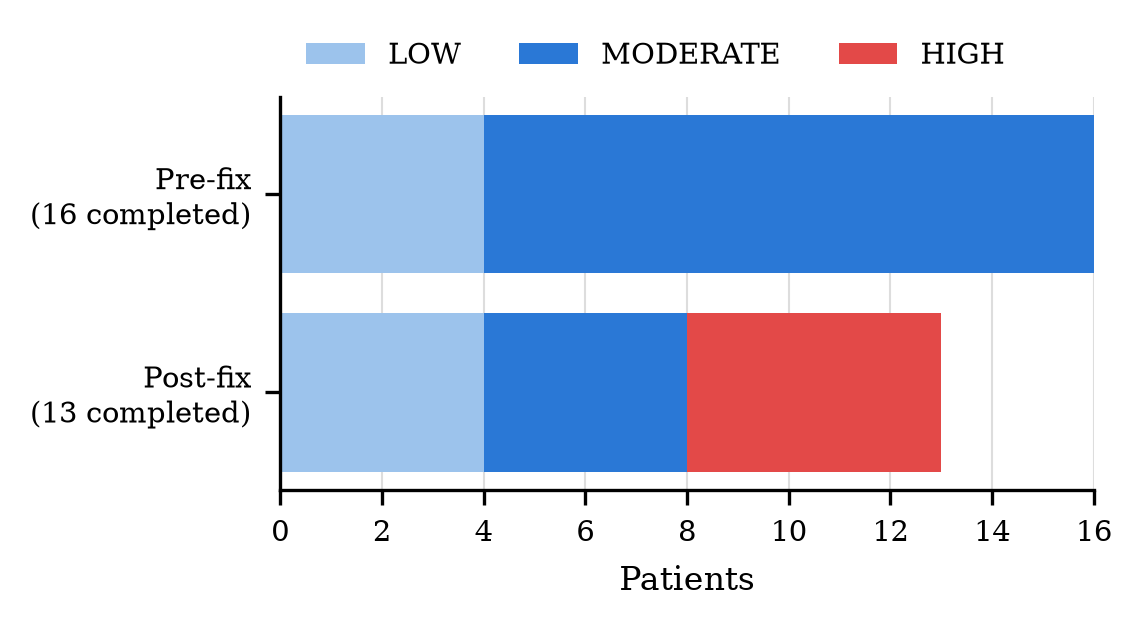
\includegraphics[width=\columnwidth]{fig_perheart_buckets.png}
\caption{Risk buckets for real PerHeart patients before and after the severity-model fix.}
\label{fig:perheart}
\end{figure}

\subsection{Measured hemodynamics (BCG, two patients)}
For two patients from a ballistocardiography dataset with echocardiographic volumes \cite{zhan2025bcg}, BCG features adjusted the twin's vascular compliance and simulated stroke volume and cardiac output were compared with measured values (Table~\ref{tab:bcg}). Simulated cardiac output was 45--46\% below measured in both; 71.3\% of patient 14's stroke-volume shortfall was already present from anthropometrics alone, before EF or BCG data entered the model. A synthetic 21-day deterioration anchored to these patients' real HR and EF was eventually classified correctly for both, but patient 14 was labeled fluid overload for days 6--10 before converging.

\begin{table}[!t]
\centering
\caption{Simulated vs.\ Measured Hemodynamics (Ratio Sim/Real)}
\label{tab:bcg}
\footnotesize
\begin{tabular}{@{}lccc@{}}
\toprule
\textbf{Subject} & \textbf{HR} & \textbf{Stroke volume} & \textbf{Cardiac output} \\
\midrule
14 & 0.94 & 0.58 & 0.54 \\
102 & 0.63 & 0.87 & 0.55 \\
\bottomrule
\end{tabular}
\end{table}

\subsection{Real-outcome tests}
Two real cohorts lack the 21-day wearable window and EF needed to run the whole twin, so only components with a non-fabricated input path were tested (Fig.~\ref{fig:auc}, Table~\ref{tab:auc}). The baseline-deficit term, a function of MAP alone, predicted in-hospital mortality in 17,129 MIMIC-IV HF ICU admissions with AUC 0.596 (95\% CI 0.585--0.608), with mortality rising monotonically from 8.9\% to 21.2\% across score deciles. On the Zigong cohort \cite{zhang2021zigong} (6-month death or readmission), the same term and a clinical-only Model~1 variant were indistinguishable from chance. As external context, an 11-of-13-variable MAGGIC score reached 0.604 and a model using laboratory panels reached 0.667, signal carried by renal and coagulation tests that a wearable-based system cannot obtain.

\begin{figure}[!t]
\centering
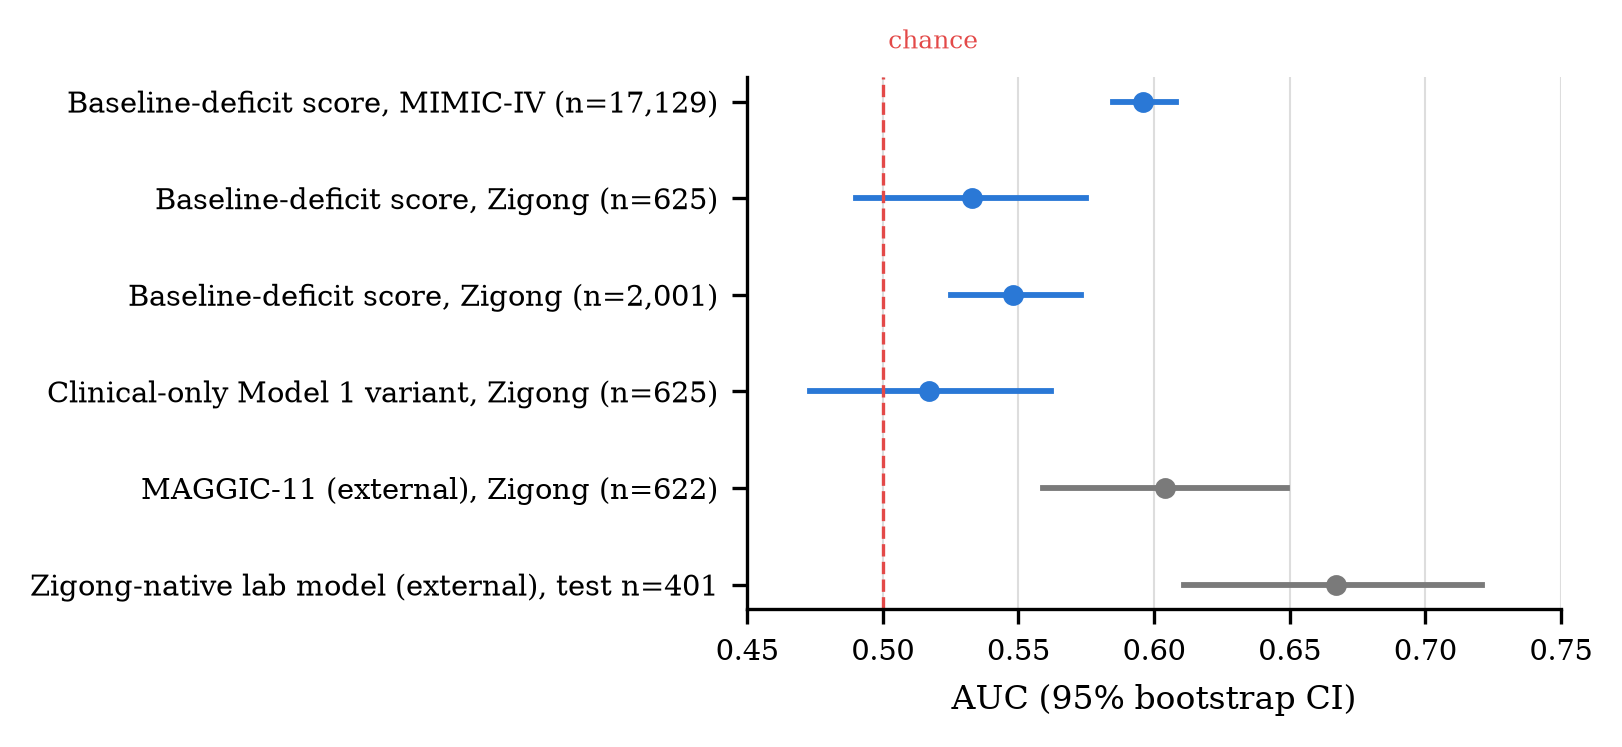
\includegraphics[width=\columnwidth]{fig_auc_forest.png}
\caption{Real-outcome discrimination. Blue: components of the twin. Grey: external benchmarks on the same cohort.}
\label{fig:auc}
\end{figure}

\begin{table}[!t]
\centering
\caption{Real-Outcome Tests (AUC, 95\% Bootstrap CI)}
\label{tab:auc}
\footnotesize
\begin{threeparttable}
\begin{tabularx}{\columnwidth}{@{}Yrl@{}}
\toprule
\textbf{Score / cohort} & \textbf{$n$} & \textbf{AUC} \\
\midrule
Baseline deficit, MIMIC-IV, in-hospital death & 17,129 & 0.596 (0.585--0.608) \\
Baseline deficit, Zigong, complete-case & 625 & 0.533 (0.490--0.575) \\
Baseline deficit, Zigong, all cleaned & 2,001 & 0.548 (0.525--0.573) \\
Clinical-only Model 1, Zigong & 625 & 0.517 (0.473--0.562) \\
MAGGIC-11 (external) \cite{pocock2013maggic}, Zigong & 622 & 0.604 (0.559--0.649) \\
Zigong lab model (external), test set & 401 & 0.667 (0.611--0.721) \\
LACE (literature) \cite{vanwalraven2010lace} & --- & $\approx$0.56--0.65 \\
\bottomrule
\end{tabularx}
\begin{tablenotes}\footnotesize
\item Zigong outcome: death or readmission within 6 months (41.3\% event rate). Bootstrap: 2,000 resamples.
\end{tablenotes}
\end{threeparttable}
\end{table}

On the synthetic batch, the risk score agreed moderately with MAGGIC computed on the same patients (Spearman $r=0.479$; tier agreement 38.5\% against $\approx$33\% by chance), indicating directional consistency rather than validity.

%=====================================================================
\section{Discussion}\label{sec:discussion}
%=====================================================================
\textbf{What the twin does well.} The pipeline runs end to end, day after day, on synthetic and real home data; it separates physiologically different presentations through mechanism rather than labels (Table~\ref{tab:phase2}); it explains alerts in terms of simulated hemodynamics; and its alert rule generalized from development to held-out seeds. Continuous state makes the twin a persistent model of a patient rather than a fresh simulation each day.

\textbf{What it does not yet do.} Three findings bound the claims. First, two of five deterioration types are invisible to the current alert because their signatures never reach the simulated hemodynamics: deconditioning by design (no acute event), and fluid overload because the scenario reduces venous compliance without adding circulating volume, which mobilizes pooled blood rather than overloading the circulation. Second, the models are sensitive to ordinary wearable noise and to clinical inputs outside their training distribution. Third, the twin's own scores do not yet predict real outcomes beyond chance, except for one component in an ICU cohort. Our results therefore support feasibility and mechanism, not clinical effectiveness.

\textbf{Lessons for building physiology-engine twins.} Every major fault in Table~\ref{tab:problems} was found by running the real system, not by offline evaluation: the NYHA skew only appeared in live inference, the CORS fault only in a browser, the resume drift only with the production modifier, and the alert mismatch only by auditing what the dashboard actually displayed. Pre-registering expectations and holding out seeds kept fixes honest, and reporting failure mechanisms rather than bare completion rates prevented a biased reading of the results.

%=====================================================================
\section{Limitations}
%=====================================================================
Training data are synthetic, although every parameter is traced to a real aggregate statistic. Pulse's native range (age 18--65, BMI 16--30) excludes most HF patients, so older patients are simulated with a proxy body. Real EF and NT-proBNP were unavailable in the replay cohort, and their defaults mask the fluid-overload mechanism. The engine's SpO$_2$ output was unusable and its ECG is a template. Pulse is unstable when disease modifiers combine with sustained exertion, which under-represents high-severity exertion scenarios in all datasets. Medication effects are not modeled: Pulse includes a validated diuretic (furosemide), making diuretic modeling feasible, but has no beta-blocker or ACE-inhibitor/ARB substances. Risk-bucket cut-points and the deterioration-rate calibration constants are engineering choices, not clinically validated thresholds. The API has no authentication and is suitable only for research use.

%=====================================================================
\section{Conclusion and Future Work}
%=====================================================================
We built and evaluated a wearable-driven heart-failure digital twin that interprets home-measurable trends through a mechanistic physiology engine and carries each patient's simulated state from day to day. It reaches high offline accuracy, runs end to end on real home-monitoring data, and, with a component-guard rule inside a three-level ALERT/WATCH/NONE decision, cuts false alarms by more than 60\% on held-out seeds while detecting three of five deterioration types. Its failures are specific and explained, which makes them actionable. Future work will (1) add a volume-loading mechanism to the fluid-overload scenario and a diuretic action using Pulse's furosemide model; (2) systematically map the engine's stability boundary across severity, scenario and body profile; (3) make the models robust to wearable noise and out-of-distribution clinical inputs; (4) personalize the twin's baseline heart rate and hemodynamics from measured data; and (5) evaluate day-by-day early warning on real longitudinal data with recorded HF events, the test that ultimately decides clinical value.

\section*{Data and Code Availability}
Synthetic data, derived results and code are in the project repository. Raw MIMIC-IV, Zigong and PerHeart files are not redistributed, in line with their access agreements; PerHeart-derived outputs are shared under CC BY-NC-SA.

\begin{thebibliography}{99}
\bibitem{james2018gbd} S. L. James \textit{et al.}, ``Global, regional, and national incidence, prevalence, and years lived with disability for 354 diseases and injuries for 195 countries and territories, 1990--2017,'' \textit{Lancet}, vol.~392, pp.~1789--1858, 2018, doi: 10.1016/S0140-6736(18)32279-7.
\bibitem{savarese2023burden} G. Savarese \textit{et al.}, ``Global burden of heart failure: A comprehensive and updated review of epidemiology,'' \textit{Cardiovasc. Res.}, vol.~118, no.~17, pp.~3272--3287, 2022, doi: 10.1093/cvr/cvac013.
\bibitem{heidenreich2022} P. A. Heidenreich \textit{et al.}, ``2022 AHA/ACC/HFSA guideline for the management of heart failure,'' \textit{Circulation}, vol.~145, 2022, doi: 10.1161/CIR.0000000000001063.
\bibitem{inglis2008telemonitoring} S. C. Inglis \textit{et al.}, ``Structured telephone support or telemonitoring programs for patients with chronic heart failure,'' \textit{Cochrane Database Syst. Rev.}, 2008, doi: 10.1002/14651858.CD007228.
\bibitem{abraham2011champion} W. T. Abraham \textit{et al.}, ``Wireless pulmonary artery haemodynamic monitoring in chronic heart failure: A randomised controlled trial,'' \textit{Lancet}, vol.~377, pp.~658--666, 2011, doi: 10.1016/S0140-6736(11)60101-3.
\bibitem{stehlik2020linkhf} J. Stehlik \textit{et al.}, ``Continuous wearable monitoring analytics predict heart failure hospitalization: The LINK-HF multicenter study,'' \textit{Circ. Heart Fail.}, vol.~13, Art.~no.~e006513, 2020, doi: 10.1161/CIRCHEARTFAILURE.119.006513.
\bibitem{gautam2022wearables} N. Gautam \textit{et al.}, ``Artificial intelligence, wearables and remote monitoring for heart failure: Current and future applications,'' \textit{Diagnostics}, vol.~12, Art.~no.~2964, 2022, doi: 10.3390/diagnostics12122964.
\bibitem{corral2020twin} J. Corral-Acero \textit{et al.}, ``The `Digital Twin' to enable the vision of precision cardiology,'' \textit{Eur. Heart J.}, vol.~41, pp.~4556--4564, 2020, doi: 10.1093/eurheartj/ehaa159.
\bibitem{coorey2022twin} G. Coorey \textit{et al.}, ``The health digital twin to tackle cardiovascular disease---A review of an emerging interdisciplinary field,'' \textit{npj Digit. Med.}, vol.~5, Art.~no.~126, 2022, doi: 10.1038/s41746-022-00640-7.
\bibitem{niederer2021scaling} S. A. Niederer \textit{et al.}, ``Scaling digital twins from the artisanal to the industrial,'' \textit{Nat. Comput. Sci.}, vol.~1, pp.~313--320, 2021, doi: 10.1038/s43588-021-00072-5.
\bibitem{gu2025hftwin} F. Gu \textit{et al.}, ``Identification of digital twins to guide interpretable AI for diagnosis and prognosis in heart failure,'' \textit{npj Digit. Med.}, vol.~8, Art.~no.~110, 2025, doi: 10.1038/s41746-025-01501-9.
\bibitem{geddes2025rhftwin} J. Geddes \textit{et al.}, ``Digital twins for noninvasively measuring predictive markers of right heart failure,'' \textit{npj Digit. Med.}, vol.~8, Art.~no.~545, 2025, doi: 10.1038/s41746-025-01920-8.
\bibitem{balasubramanyam2025twin} A. Balasubramanyam \textit{et al.}, ``A cardiovascular modeling framework for enabling personalized healthcare: A digital twin approach,'' in \textit{Proc. IEEE 13th Int. Conf. Healthcare Informatics (ICHI)}, 2025, pp.~478--489, doi: 10.1109/ICHI64645.2025.00062.
\bibitem{bray2019pulse} A. Bray \textit{et al.}, ``Pulse Physiology Engine: An open-source software platform for computational modeling of human medical simulation,'' \textit{SN Compr. Clin. Med.}, vol.~1, pp.~362--377, 2019, doi: 10.1007/s42399-019-00053-w.
\bibitem{pocock2013maggic} S. J. Pocock \textit{et al.}, ``Predicting survival in heart failure: A risk score based on 39\,372 patients from 30 studies,'' \textit{Eur. Heart J.}, vol.~34, pp.~1404--1413, 2013, doi: 10.1093/eurheartj/ehs337.
\bibitem{vanwalraven2010lace} C. van Walraven \textit{et al.}, ``Derivation and validation of an index to predict early death or unplanned readmission after discharge from hospital to the community,'' \textit{CMAJ}, vol.~182, no.~6, pp.~551--557, 2010, doi: 10.1503/cmaj.091117.
\bibitem{breiman2001rf} L. Breiman, ``Random forests,'' \textit{Mach. Learn.}, vol.~45, no.~1, pp.~5--32, 2001, doi: 10.1023/A:1010933404324.
\bibitem{pedregosa2011sklearn} F. Pedregosa \textit{et al.}, ``Scikit-learn: Machine learning in Python,'' \textit{J. Mach. Learn. Res.}, vol.~12, pp.~2825--2830, 2011.
\bibitem{chen2016xgboost} T. Chen and C. Guestrin, ``XGBoost: A scalable tree boosting system,'' in \textit{Proc. 22nd ACM SIGKDD Int. Conf. Knowl. Discov. Data Min.}, 2016, pp.~785--794, doi: 10.1145/2939672.2939785.
\bibitem{johnson2023mimiciv} A. E. W. Johnson \textit{et al.}, ``MIMIC-IV, a freely accessible electronic health record dataset,'' \textit{Sci. Data}, vol.~10, Art.~no.~1, 2023, doi: 10.1038/s41597-022-01899-x.
\bibitem{goldberger2000physionet} A. L. Goldberger \textit{et al.}, ``PhysioBank, PhysioToolkit, and PhysioNet: Components of a new research resource for complex physiologic signals,'' \textit{Circulation}, vol.~101, no.~23, pp.~e215--e220, 2000, doi: 10.1161/01.CIR.101.23.e215.
\bibitem{chicco2020hf} D. Chicco and G. Jurman, ``Machine learning can predict survival of patients with heart failure from serum creatinine and ejection fraction alone,'' \textit{BMC Med. Inform. Decis. Mak.}, vol.~20, Art.~no.~16, 2020, doi: 10.1186/s12911-020-1023-5.
\bibitem{kolakowski2026perheart} M. Kolakowski \textit{et al.}, ``Multimodal dataset of in-home physiological and inertial measurements from older heart failure patients,'' \textit{Data}, vol.~11, Art.~no.~106, 2026, doi: 10.3390/data11050106.
\bibitem{zhang2021zigong} Z. Zhang \textit{et al.}, ``Electronic healthcare records and external outcome data for hospitalized patients with heart failure,'' \textit{Sci. Data}, vol.~8, Art.~no.~46, 2021, doi: 10.1038/s41597-021-00835-9.
\bibitem{zhan2025bcg} J. Zhan \textit{et al.}, ``A multi-pathology ballistocardiogram dataset for cardiac function monitoring and arrhythmia assessment,'' figshare, 2025, doi: 10.6084/m9.figshare.28416896.
\bibitem{rcp2017news2} Royal College of Physicians, ``National Early Warning Score (NEWS) 2: Standardising the assessment of acute-illness severity in the NHS,'' London, U.K., 2017.
\bibitem{vincent2013shock} J.-L. Vincent and D. De Backer, ``Circulatory shock,'' \textit{N. Engl. J. Med.}, vol.~369, no.~18, pp.~1726--1734, 2013, doi: 10.1056/NEJMra1208943.
\bibitem{nohria2002management} A. Nohria, E. Lewis, and L. W. Stevenson, ``Medical management of advanced heart failure,'' \textit{JAMA}, vol.~287, no.~5, pp.~628--640, 2002, doi: 10.1001/jama.287.5.628.
\bibitem{baran2019scai} D. A. Baran \textit{et al.}, ``SCAI clinical expert consensus statement on the classification of cardiogenic shock,'' \textit{Catheter. Cardiovasc. Interv.}, vol.~94, pp.~29--37, 2019, doi: 10.1002/ccd.28329.
\end{thebibliography}

\end{document}
